\documentclass[]{article}
\usepackage{lmodern}
\usepackage{amssymb,amsmath}
\usepackage{ifxetex,ifluatex}
\usepackage{fixltx2e} % provides \textsubscript
\ifnum 0\ifxetex 1\fi\ifluatex 1\fi=0 % if pdftex
  \usepackage[T1]{fontenc}
  \usepackage[utf8]{inputenc}
\else % if luatex or xelatex
  \ifxetex
    \usepackage{mathspec}
  \else
    \usepackage{fontspec}
  \fi
  \defaultfontfeatures{Ligatures=TeX,Scale=MatchLowercase}
\fi
% use upquote if available, for straight quotes in verbatim environments
\IfFileExists{upquote.sty}{\usepackage{upquote}}{}
% use microtype if available
\IfFileExists{microtype.sty}{%
\usepackage{microtype}
\UseMicrotypeSet[protrusion]{basicmath} % disable protrusion for tt fonts
}{}
\usepackage[margin=1in]{geometry}
\usepackage{hyperref}
\hypersetup{unicode=true,
            pdftitle={Comparaciones posthoc y diseños anidados},
            pdfborder={0 0 0},
            breaklinks=true}
\urlstyle{same}  % don't use monospace font for urls
\usepackage{color}
\usepackage{fancyvrb}
\newcommand{\VerbBar}{|}
\newcommand{\VERB}{\Verb[commandchars=\\\{\}]}
\DefineVerbatimEnvironment{Highlighting}{Verbatim}{commandchars=\\\{\}}
% Add ',fontsize=\small' for more characters per line
\usepackage{framed}
\definecolor{shadecolor}{RGB}{248,248,248}
\newenvironment{Shaded}{\begin{snugshade}}{\end{snugshade}}
\newcommand{\KeywordTok}[1]{\textcolor[rgb]{0.13,0.29,0.53}{\textbf{#1}}}
\newcommand{\DataTypeTok}[1]{\textcolor[rgb]{0.13,0.29,0.53}{#1}}
\newcommand{\DecValTok}[1]{\textcolor[rgb]{0.00,0.00,0.81}{#1}}
\newcommand{\BaseNTok}[1]{\textcolor[rgb]{0.00,0.00,0.81}{#1}}
\newcommand{\FloatTok}[1]{\textcolor[rgb]{0.00,0.00,0.81}{#1}}
\newcommand{\ConstantTok}[1]{\textcolor[rgb]{0.00,0.00,0.00}{#1}}
\newcommand{\CharTok}[1]{\textcolor[rgb]{0.31,0.60,0.02}{#1}}
\newcommand{\SpecialCharTok}[1]{\textcolor[rgb]{0.00,0.00,0.00}{#1}}
\newcommand{\StringTok}[1]{\textcolor[rgb]{0.31,0.60,0.02}{#1}}
\newcommand{\VerbatimStringTok}[1]{\textcolor[rgb]{0.31,0.60,0.02}{#1}}
\newcommand{\SpecialStringTok}[1]{\textcolor[rgb]{0.31,0.60,0.02}{#1}}
\newcommand{\ImportTok}[1]{#1}
\newcommand{\CommentTok}[1]{\textcolor[rgb]{0.56,0.35,0.01}{\textit{#1}}}
\newcommand{\DocumentationTok}[1]{\textcolor[rgb]{0.56,0.35,0.01}{\textbf{\textit{#1}}}}
\newcommand{\AnnotationTok}[1]{\textcolor[rgb]{0.56,0.35,0.01}{\textbf{\textit{#1}}}}
\newcommand{\CommentVarTok}[1]{\textcolor[rgb]{0.56,0.35,0.01}{\textbf{\textit{#1}}}}
\newcommand{\OtherTok}[1]{\textcolor[rgb]{0.56,0.35,0.01}{#1}}
\newcommand{\FunctionTok}[1]{\textcolor[rgb]{0.00,0.00,0.00}{#1}}
\newcommand{\VariableTok}[1]{\textcolor[rgb]{0.00,0.00,0.00}{#1}}
\newcommand{\ControlFlowTok}[1]{\textcolor[rgb]{0.13,0.29,0.53}{\textbf{#1}}}
\newcommand{\OperatorTok}[1]{\textcolor[rgb]{0.81,0.36,0.00}{\textbf{#1}}}
\newcommand{\BuiltInTok}[1]{#1}
\newcommand{\ExtensionTok}[1]{#1}
\newcommand{\PreprocessorTok}[1]{\textcolor[rgb]{0.56,0.35,0.01}{\textit{#1}}}
\newcommand{\AttributeTok}[1]{\textcolor[rgb]{0.77,0.63,0.00}{#1}}
\newcommand{\RegionMarkerTok}[1]{#1}
\newcommand{\InformationTok}[1]{\textcolor[rgb]{0.56,0.35,0.01}{\textbf{\textit{#1}}}}
\newcommand{\WarningTok}[1]{\textcolor[rgb]{0.56,0.35,0.01}{\textbf{\textit{#1}}}}
\newcommand{\AlertTok}[1]{\textcolor[rgb]{0.94,0.16,0.16}{#1}}
\newcommand{\ErrorTok}[1]{\textcolor[rgb]{0.64,0.00,0.00}{\textbf{#1}}}
\newcommand{\NormalTok}[1]{#1}
\usepackage{graphicx,grffile}
\makeatletter
\def\maxwidth{\ifdim\Gin@nat@width>\linewidth\linewidth\else\Gin@nat@width\fi}
\def\maxheight{\ifdim\Gin@nat@height>\textheight\textheight\else\Gin@nat@height\fi}
\makeatother
% Scale images if necessary, so that they will not overflow the page
% margins by default, and it is still possible to overwrite the defaults
% using explicit options in \includegraphics[width, height, ...]{}
\setkeys{Gin}{width=\maxwidth,height=\maxheight,keepaspectratio}
\IfFileExists{parskip.sty}{%
\usepackage{parskip}
}{% else
\setlength{\parindent}{0pt}
\setlength{\parskip}{6pt plus 2pt minus 1pt}
}
\setlength{\emergencystretch}{3em}  % prevent overfull lines
\providecommand{\tightlist}{%
  \setlength{\itemsep}{0pt}\setlength{\parskip}{0pt}}
\setcounter{secnumdepth}{0}
% Redefines (sub)paragraphs to behave more like sections
\ifx\paragraph\undefined\else
\let\oldparagraph\paragraph
\renewcommand{\paragraph}[1]{\oldparagraph{#1}\mbox{}}
\fi
\ifx\subparagraph\undefined\else
\let\oldsubparagraph\subparagraph
\renewcommand{\subparagraph}[1]{\oldsubparagraph{#1}\mbox{}}
\fi

%%% Use protect on footnotes to avoid problems with footnotes in titles
\let\rmarkdownfootnote\footnote%
\def\footnote{\protect\rmarkdownfootnote}

%%% Change title format to be more compact
\usepackage{titling}

% Create subtitle command for use in maketitle
\newcommand{\subtitle}[1]{
  \posttitle{
    \begin{center}\large#1\end{center}
    }
}

\setlength{\droptitle}{-2em}
  \title{Comparaciones posthoc y diseños anidados}
  \pretitle{\vspace{\droptitle}\centering\huge}
  \posttitle{\par}
  \author{}
  \preauthor{}\postauthor{}
  \predate{\centering\large\emph}
  \postdate{\par}
  \date{March 31, 2018}


\begin{document}
\maketitle

{
\setcounter{tocdepth}{2}
\tableofcontents
}
\subsection{Comparaciones posthoc}\label{comparaciones-posthoc}

Como ya vimos en los prácticos anteriores, un ANOVA sólo puede decirnos
si hay diferencias entre grupos, sin embargo no nos dira entre que
grupos hay diferencias, es para esto que existen las pruebas posthoc. En
el práctico de hoy veremos dos tipos de comparaciones posthoc, la prueba
honesta de diferencias significativas de Tukey (función
\texttt{TukeyHSD} en R), y los ajustes de valores de p para
comparaciones multiples (función \texttt{pairwise.t.test} en R), de las
cuales la de Bonferroni es la más habitual.

\subsubsection{Prueba honesta de diferencias significativas de
Tukey}\label{prueba-honesta-de-diferencias-significativas-de-tukey}

\paragraph{Ejemplo ancho de spealo en el genero
Iris}\label{ejemplo-ancho-de-spealo-en-el-genero-iris}

Como vimos en nuestro ejemplo de la guía número 3 (Análisis exploratorio
y el primer ANOVA), el ANOVA para determinar si hay diferencias en el
ancho de sépalo entre las diferentes especies del genero \emph{Iris},
son significativas:

\begin{Shaded}
\begin{Highlighting}[]
\KeywordTok{summary}\NormalTok{(}\KeywordTok{aov}\NormalTok{(Sepal.Width }\OperatorTok{~}\StringTok{ }\NormalTok{Species, }\DataTypeTok{data =}\NormalTok{ iris))}
\end{Highlighting}
\end{Shaded}

\begin{verbatim}
##              Df Sum Sq Mean Sq F value Pr(>F)    
## Species       2  11.35   5.672   49.16 <2e-16 ***
## Residuals   147  16.96   0.115                   
## ---
## Signif. codes:  0 '***' 0.001 '**' 0.01 '*' 0.05 '.' 0.1 ' ' 1
\end{verbatim}

Pero este análisis no nos dice en tre que especies encontramos estas
diferencias, para esto, podemos realizar una prueba honesta de
diferencias significativas de Tukey, para esto utilizamos la función
\texttt{TukeyHSD} y usamos como argumento un ANOVA ya ajustado

\begin{Shaded}
\begin{Highlighting}[]
\NormalTok{AnovaSepalo <-}\StringTok{ }\KeywordTok{aov}\NormalTok{(Sepal.Width }\OperatorTok{~}\StringTok{ }\NormalTok{Species, }\DataTypeTok{data =}\NormalTok{ iris)}
\KeywordTok{TukeyHSD}\NormalTok{(AnovaSepalo)}
\end{Highlighting}
\end{Shaded}

\begin{verbatim}
##   Tukey multiple comparisons of means
##     95% family-wise confidence level
## 
## Fit: aov(formula = Sepal.Width ~ Species, data = iris)
## 
## $Species
##                        diff         lwr        upr     p adj
## versicolor-setosa    -0.658 -0.81885528 -0.4971447 0.0000000
## virginica-setosa     -0.454 -0.61485528 -0.2931447 0.0000000
## virginica-versicolor  0.204  0.04314472  0.3648553 0.0087802
\end{verbatim}

\subsubsection{Ajustes de valores de p para comparaciones
multiples}\label{ajustes-de-valores-de-p-para-comparaciones-multiples}

\paragraph{Ajuste de Bonferroni}\label{ajuste-de-bonferroni}

Cuando realizamos multiples comparaciones pareadas entre grupos, la
probabilidad de encontrar diferencias significativas cuando no los hay
(error tipo I), aumenta a una tasa dada por la siguiente fórmula:

\[\alpha_{ajustado} = 1 - (1 -\alpha)^n\] Donde \(\alpha\) es la
probabilidad de cometer un error tipo I que estamos dispuestos a aceptar
(tipicamente 0.05), y \(n\) es el numero de pruebas independientes a
realizar.

Con esto según el ajuste de Bonferroni, nuestro p critico para
determinar diferencias significativas cambia segun la siguiente fórmula
(Tukey 1977)

\[p-critico_{ajustado} = 1 - (1 -\alpha)^{1/n}\] El ajuste de
Bonferroni, sin embargo al disminuir los errores de tipo I, aumenta los
errores de tipo II (Morgan 2007). En ese sentido, la función de R
\texttt{pairwise.t.test}, nos permite utilizar varios ajustes menos
conservadores incluyendo los de Holm (1979), Hochberg (1988), Hommel
(1988), Benjamini \& Hochberg (1995) o el de Benjamini \& Yekutieli
(2001)

\paragraph{Ejemplo ancho de spealo en el genero
Iris}\label{ejemplo-ancho-de-spealo-en-el-genero-iris-1}

Volviendo al mismo ejemplo que usamos en la prueba de Tukey, mostraremos
los valores de p determinados para comparaciones multiples de el ancho
de sepalo sin ajuste y con diversos ajustes que encontramos en el la
función \texttt{pairwise.t.test}

\subparagraph{Sin ajuste}\label{sin-ajuste}

\begin{Shaded}
\begin{Highlighting}[]
\KeywordTok{pairwise.t.test}\NormalTok{(}\DataTypeTok{x =}\NormalTok{ airquality}\OperatorTok{$}\NormalTok{Ozone, }\DataTypeTok{g =}\NormalTok{ airquality}\OperatorTok{$}\NormalTok{Month, }\DataTypeTok{p.adj =} \StringTok{"none"}\NormalTok{)}
\end{Highlighting}
\end{Shaded}

\begin{verbatim}
## 
##  Pairwise comparisons using t tests with pooled SD 
## 
## data:  airquality$Ozone and airquality$Month 
## 
##   5       6       7       8      
## 6 0.60877 -       -       -      
## 7 2.9e-05 0.01023 -       -      
## 8 1.9e-05 0.00831 0.91744 -      
## 9 0.32545 0.85838 0.00070 0.00048
## 
## P value adjustment method: none
\end{verbatim}

\subparagraph{Ajuste de Bonferroni}\label{ajuste-de-bonferroni-1}

\begin{Shaded}
\begin{Highlighting}[]
\KeywordTok{pairwise.t.test}\NormalTok{(}\DataTypeTok{x =}\NormalTok{ airquality}\OperatorTok{$}\NormalTok{Ozone, }\DataTypeTok{g =}\NormalTok{ airquality}\OperatorTok{$}\NormalTok{Month, }\DataTypeTok{p.adj =} \StringTok{"bonf"}\NormalTok{)}
\end{Highlighting}
\end{Shaded}

\begin{verbatim}
## 
##  Pairwise comparisons using t tests with pooled SD 
## 
## data:  airquality$Ozone and airquality$Month 
## 
##   5       6       7       8      
## 6 1.00000 -       -       -      
## 7 0.00029 0.10225 -       -      
## 8 0.00019 0.08312 1.00000 -      
## 9 1.00000 1.00000 0.00697 0.00485
## 
## P value adjustment method: bonferroni
\end{verbatim}

\subparagraph{Ajuste de Holm}\label{ajuste-de-holm}

\begin{Shaded}
\begin{Highlighting}[]
\KeywordTok{pairwise.t.test}\NormalTok{(}\DataTypeTok{x =}\NormalTok{ airquality}\OperatorTok{$}\NormalTok{Ozone, }\DataTypeTok{g =}\NormalTok{ airquality}\OperatorTok{$}\NormalTok{Month, }\DataTypeTok{p.adj =} \StringTok{"holm"}\NormalTok{)}
\end{Highlighting}
\end{Shaded}

\begin{verbatim}
## 
##  Pairwise comparisons using t tests with pooled SD 
## 
## data:  airquality$Ozone and airquality$Month 
## 
##   5       6       7       8      
## 6 1.00000 -       -       -      
## 7 0.00026 0.05113 -       -      
## 8 0.00019 0.04987 1.00000 -      
## 9 1.00000 1.00000 0.00488 0.00388
## 
## P value adjustment method: holm
\end{verbatim}

\subparagraph{Ajuste de Hommel}\label{ajuste-de-hommel}

\begin{Shaded}
\begin{Highlighting}[]
\KeywordTok{pairwise.t.test}\NormalTok{(}\DataTypeTok{x =}\NormalTok{ airquality}\OperatorTok{$}\NormalTok{Ozone, }\DataTypeTok{g =}\NormalTok{ airquality}\OperatorTok{$}\NormalTok{Month, }\DataTypeTok{p.adj =} \StringTok{"hommel"}\NormalTok{)}
\end{Highlighting}
\end{Shaded}

\begin{verbatim}
## 
##  Pairwise comparisons using t tests with pooled SD 
## 
## data:  airquality$Ozone and airquality$Month 
## 
##   5       6       7       8      
## 6 0.91744 -       -       -      
## 7 0.00026 0.05113 -       -      
## 8 0.00018 0.04156 0.91744 -      
## 9 0.91744 0.91744 0.00488 0.00339
## 
## P value adjustment method: hommel
\end{verbatim}

\subparagraph{Diferencias}\label{diferencias}

Se observa como sin ajustar hay 6 pares de meses que tienen diferencias,
en contraste con 4 pares de meses con el ajuste de Bonferroni, y 5 con
los otros métodos de ajuste de valor de p.

\subsection{Diseños anidados}\label{disenos-anidados}

Los diseños anidados ocurren cuando queremos estudiar el efecto de un
factor, pero dentro de las muestras existe un segundo factor que puede
afectar nuestros análisis, por ejemplo si volvemos a el caso en

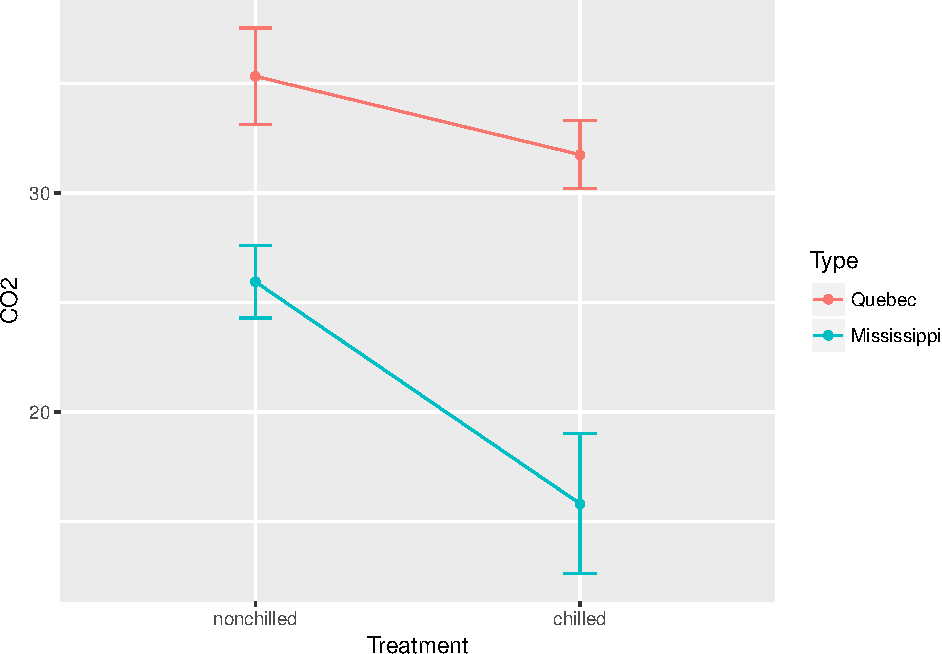
\includegraphics{Guia6_files/figure-latex/unnamed-chunk-7-1.pdf}

\begin{verbatim}
##              Df Sum Sq Mean Sq F value Pr(>F)    
## Var1          2   7000    3500 206.611 <2e-16 ***
## Var2          1      4       4   0.227  0.634    
## Var1:Var2     2      0       0   0.000  1.000    
## Residuals   174   2948      17                   
## ---
## Signif. codes:  0 '***' 0.001 '**' 0.01 '*' 0.05 '.' 0.1 ' ' 1
\end{verbatim}

\begin{verbatim}
##              Df Sum Sq Mean Sq F value Pr(>F)    
## Var1          2      2       1   0.068  0.935    
## Var2          1   4500    4500 281.208 <2e-16 ***
## Var1:Var2     2      6       3   0.203  0.816    
## Residuals   174   2784      16                   
## ---
## Signif. codes:  0 '***' 0.001 '**' 0.01 '*' 0.05 '.' 0.1 ' ' 1
\end{verbatim}

\begin{verbatim}
##              Df Sum Sq Mean Sq F value Pr(>F)    
## Var1          2   1828   913.9   57.11 <2e-16 ***
## Var2          1   3125  3125.0  195.28 <2e-16 ***
## Var1:Var2     2   1925   962.4   60.14 <2e-16 ***
## Residuals   174   2784    16.0                   
## ---
## Signif. codes:  0 '***' 0.001 '**' 0.01 '*' 0.05 '.' 0.1 ' ' 1
\end{verbatim}

\begin{verbatim}
##              Df Sum Sq Mean Sq F value   Pr(>F)    
## Var1          2    294     147   9.175 0.000163 ***
## Var2          1      0       0   0.000 1.000000    
## Var1:Var2     2   7130    3565 222.769  < 2e-16 ***
## Residuals   174   2784      16                     
## ---
## Signif. codes:  0 '***' 0.001 '**' 0.01 '*' 0.05 '.' 0.1 ' ' 1
\end{verbatim}

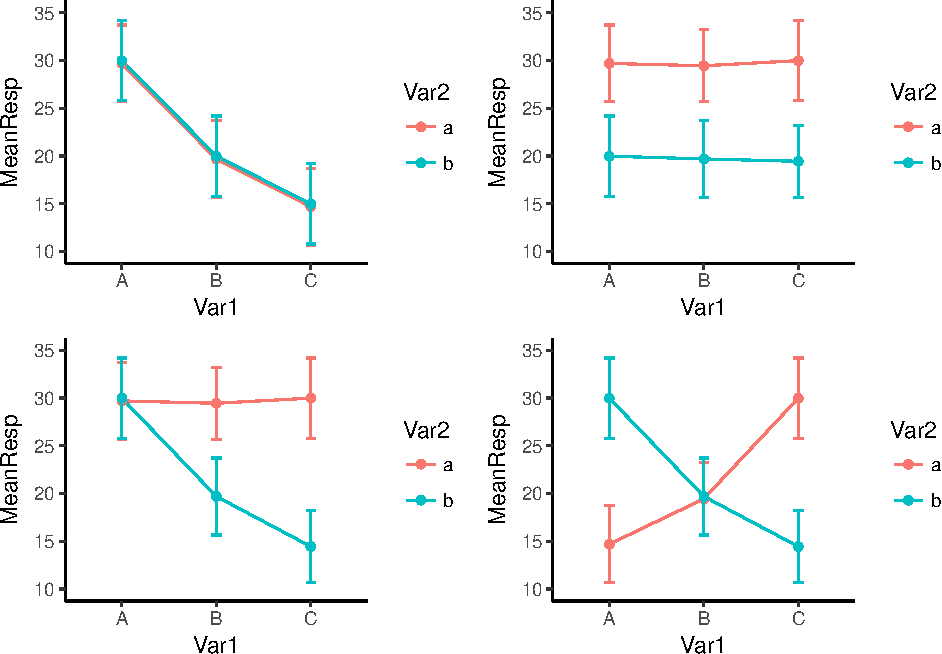
\includegraphics{Guia6_files/figure-latex/unnamed-chunk-8-1.pdf}

\subsection*{Referencias}\label{referencias}
\addcontentsline{toc}{subsection}{Referencias}

\hypertarget{refs}{}
\hypertarget{ref-morgan2007p}{}
Morgan, John F. 2007. ``P Value Fetishism and Use of the Bonferroni
Adjustment.'' \emph{Evidence-Based Mental Health} 10 (2). BMJ Publishing
Group LTD: 34.

\hypertarget{ref-tukey1977some}{}
Tukey, John W. 1977. ``Some Thoughts on Clinical Trials, Especially
Problems of Multiplicity.'' \emph{Science} 198 (4318). American
Asociation for the Advancement of Science: 679--84.


\end{document}
